\documentclass[a4paper, 12pt, twoside]{article}
\usepackage[top=24mm, bottom=24mm, inner=35mm, outer=24mm]{geometry}
\usepackage[backend=biber]{biblatex}
\usepackage{graphicx}
\usepackage{caption}
\usepackage{hyperref}
\usepackage{tabularx}
\usepackage[autostyle]{csquotes}  

% Define \fullref command to reference both number and name of section
\newcommand*{\fullref}[1]{\ref{#1} \nameref{#1}}

%Package stuff for the user stories
\usepackage{framed}
\usepackage{tikz}
\usetikzlibrary{decorations.pathmorphing,calc,positioning,shapes,shadows,arrows}
\tikzstyle{abstract}=[rectangle, draw=black, rounded corners, fill=gray!80, drop shadow,
        text centered, anchor=north, text=white, text width=3cm]
\tikzstyle{comment}=[rectangle, draw=black, rounded corners, fill=white, drop shadow,
        text centered, anchor=north, text=white, text width=3cm]
\tikzstyle{myarrow}=[->, >=open triangle 90, thick]
\tikzstyle{line}=[-, thick]
\pgfmathsetseed{1} % To have predictable results
% Define a background layer, in which the parchment shape is drawn
\pgfdeclarelayer{background}
\pgfsetlayers{background,main}
% define styles for the normal border and the torn border
\tikzset{
  normal border/.style={orange!30!black!10, decorate
     }}

     % Macro to draw the shape behind the text, when it fits completly in the
% page
\def\parchmentframe#1{
\tikz{
  \node[inner sep=2em] (A) {#1};  % Draw the text of the node
  \begin{pgfonlayer}{background}  % Draw the shape behind
  \fill[normal border]
        (A.south east) -- (A.south west) --
        (A.north west) -- (A.north east) -- cycle;
  \end{pgfonlayer}}}

% Macro to draw the shape, when the text will continue in next page
\def\parchmentframetop#1{
\tikz{
  \node[inner sep=2em] (A) {#1};    % Draw the text of the node
  \begin{pgfonlayer}{background}
  \fill[normal border]              % Draw the ``complete shape'' behind
        (A.south east) -- (A.south west) --
        (A.north west) -- (A.north east) -- cycle;
  \end{pgfonlayer}}}

% Macro to draw the shape, when the text continues from previous page
\def\parchmentframebottom#1{
\tikz{
  \node[inner sep=2em] (A) {#1};   % Draw the text of the node
  \begin{pgfonlayer}{background}
  \fill[normal border]             % Draw the ``complete shape'' behind
        (A.south east) -- (A.south west) --
        (A.north west) -- (A.north east) -- cycle;
  \end{pgfonlayer}}}

% Macro to draw the shape, when both the text continues from previous page
% and it will continue in next page
\def\parchmentframemiddle#1{
\tikz{
  \node[inner sep=2em] (A) {#1};   % Draw the text of the node
  \begin{pgfonlayer}{background}
  \fill[normal border]             % Draw the ``complete shape'' behind
        (A.south east) -- (A.south west) --
        (A.north west) -- (A.north east) -- cycle;
  \end{pgfonlayer}}}

% Define the environment which puts the frame
% In this case, the environment also accepts an argument with an optional
% title (which defaults to ``Example'', which is typeset in a box overlaid
% on the top border
\newenvironment{parchment}[1][Example]{%
  \def\FrameCommand{\parchmentframe}%
  \def\FirstFrameCommand{\parchmentframetop}%
  \def\LastFrameCommand{\parchmentframebottom}%
  \def\MidFrameCommand{\parchmentframemiddle}%
  \vskip\baselineskip
  \MakeFramed {\FrameRestore}
  \noindent\tikz\node[inner sep=1ex, draw=black!20,fill=white,
          anchor=west, overlay] at (0em, 2em) {\sffamily#1};\par}%
{\endMakeFramed}

%End User story package stuff

\addbibresource{report.bib}
\nocite{*}

\newcommand{\userstory}[4]{
	\begin{parchment}[User Story: #1]
	\noindent\emph{\textbf{AS A}} {\small #2}\\*\emph{\textbf{I WANT}} {\small #3}\\*\emph{\textbf{SO THAT}} {\small #4}
	\end{parchment}
}

\begin{document}

\begin{titlepage}

	\center

	{\large ELECTRONICS AND COMPUTER SCIENCE}\\[0.2cm]
	{\large FACULTY OF PHYSICAL SCIENCES AND ENGINEERING}\\[0.2cm]
	{\large UNIVERSITY OF SOUTHAMPTON}\\[3cm]

	{\Large Peter Prince}\\[0.2cm]
	{\Large James Robinson}\\[0.2cm]
	{\Large Charles Sherman}\\[0.2cm]
	{\Large Andrew Sullivan}\\[1cm]
	{\Large \today}\\[3cm]

	{\LARGE Aeronautical Event Service}\\[3cm]

	{\large Project Supervisor: Dr Robert Walters}\\[0.2cm]
	{\large Second Examiner: Professor Mike Wald}\\[2.5cm]

	{\large A project report submitted for the award of}\\[0.2cm]
	{\Large MEng Computer Science}

\end{titlepage}

\begin{abstract}

\end{abstract}

\newpage

\section*{Acknowledgements}

\newpage

\tableofcontents
\newpage

\listoffigures
\newpage

\section{Introduction}
\label{sec:introduction}

The project customer was Snowflake Software, a company that works in geographical data exchange services. The focus of this project is the exchange of aeronautical data between flight planners and data publishers such as the Federal Notam Service and the Aeronautical Information Service. Snowflake were planning to implement a data exchange service for clients that would allow consumers to receive aeronautical data in the form of `Notice to Airmen', using a push notification service. The group was given the task: ``To demonstrate the feasibility of using Publish/Subscribe to communicate relevant NOTAMs to flight planners''. In practice, this translated to exploring what architectures existed that could be used to implement a push notification system, and which of those would work with the requested standard of WSN.

\newpage

\section{Project Description}
\subsection{Motivation}
\label{sec:intro_motivation}
Pilots need to be notified of hazards and events that may require them to make changes to their flight plan. Examples of such events includes: closed runways, restricted airspaces, extreme weather conditions, and even the presence of migrating birds through an airspace. Currently, flight planners receive such information by pulling all current NOTAM's, or `Notice to Airmen', and must manually sort through them to find only the notices which are relevant to their flight, which is extremely time consuming. The efficiency of this task could be improved dramatically if the filtering were performed automatically, using defined geographic regions and time frames. The aeronautics industry uses WSN as their preferred standard, so our customer required us to work to this standard or WS-Events.

\subsection{Customer}
\label{sec:intro_customer}

The customer for this project was Snowflake Software, a company focused on open data exchange, and various data mapping products. Within sprint meetings, the company was represented by Eddie Curtis, who expressed the feature requests and gave feedback, representing the product owner, whist Adrian McKenzie served as the scrum master, guiding sprint meetings and ensuring the team were able to work effectively and without impediment.

\subsection{Goals}
\label{sec:intro_goals}

The vision, as stated by Snowflake, was ``To develop a proof of concept push event service for delivering digital NOTAM updates to pilots; to demonstrate the feasibility of using Publish/Subscribe to communicate relevant NOTAMs to flight planners''. From this vision, the goal of the software produced over the course of the project was to explore options and find methods to limit the incoming data to a flight planner to only relevant data by utilising a publish and subscribe model, removing the need for manual filtering and the pulling of relevant NOTAMs by pilots.

The subscriptions to this service had to be based on the relevancy of NOTAMs to the recipients. This relevancy was determined by geographic data, such as departure and arrival airports, and more complex temporal queries, for example, limiting NOTAM to ones relevant only during the course of the flight. The software was required to use open standards for the publish and subscribe architecture, for example: OASIS Web Services Notification or WSN. The software also had to be capable of handling an estimated 10,000 messages per day. These messages come from two sources: the Federal NOTAM Service, which publishes a baseline NOTAM every 28 days, and updated delta files which arrive every 15 minutes.

\subsubsection{Project Goals}
\begin{enumerate}
\item Capable of parsing XML documents from the AIXM schema.
\item Capable of basic filtering of NOTAMs based on simple text fields such as airport names.
\item Capable of temporal filtering of NOTAMs.
\item Capable of receiving and handling subscriptions from consumers.
\item Capable of publishing parsed NOTAMs to relevant subscribers.
\item Produced utilising exclusively open-source libraries.
\item Using WS-Notifications to securely communicate all NOTAMs.
\item Able to handle 10,000 messages per day.
\item Store and update baselines to provide to consumers upon connection.
\end{enumerate}

\subsubsection{Additional Goals}
\begin{enumerate}
\item Spatial filtering of NOTAMs based on distances from points.
\item Spatial filtering of NOTAMs based on locations within bounding boxes.
\item Retrieve GPS co-ordinates for airports and airspaces from Snowflake's Global Aerodromes web service.
\item Enriching NOTAMs with GPS co-ordinates to allow for faster spatial filtering.
\item Handle cases where the Global Aerodromes service does not contain a designator for a location.
\end{enumerate}

\subsubsection{Project Scope Changes}
In the opening meeting, the initial project goals were set out by the scrum master, Adrian, and product owner, Eddie. Several meetings later, this list of requirements was updated, making spatial filtering a major focus for the project and temporal filtering an extension goal to complete if time permitted. As most of the groundwork for both filtering types could be reused, both were completed.

The storing and provision of baselines ceased to be a requirement after a few meetings, when it was revealed that Snowflake already possessed a service which provided updated NOTAM baselines and so this functionality was not required of any system produced in the course of this project.

\subsection{Deliverables}
\label{sec:plan_deliverables}

The deliverables for the project were dictated both by the requirements of our customer and the module requirements. Snowflake required the production of a proof of concept service which fulfilled their requirements, whereas the module required several more deliverables.

\begin{itemize}
\item Functioning proof of concept service
\item Example project of service with consumer
\item Final group report
\item Final individual report
\item Progress seminar 1
\item Progress seminar 2
\item Final presentation
\item Group design project poster
\end{itemize}

The deliverables for the customer included both the functioning service which serves as a proof of concept for publish/subscribe-based NOTAM services and an example project for demonstrating its functionality in the final presentation.

In the first progress seminar, a description of the project goals was presented, along with our plans for how to proceed from that point onwards. The second seminar contained a brief overview of the project for the second examiner, a description of all previous work completed and our plans for the remainder of our time on the project.

\section{Background Information}

\subsection{NOTAMs}
\label{sec:bg_notams}
A `notice to airmen' (NOTAM), is a notice given to airmen about events in a particular airspace or at a particular airport. The events may be hazards that have to be avoided, such as dangerous weather, or updates on runway closures, which may or may not be relevant to the flight. They're used by pilots and flight planners to notify them about events that might affect the safety of their flight. NOTAMs are distributed by various aviation authorities around the world and are generally received by pilots and flight planners by pull notifications.

The NOTAMs are delivered as deltas from a baseline of data. For instance, the latest baseline data may indicate that a particular runway has been closed indefinitely but a pilot may be told via a NOTAM that the runway has been reopened, overriding the baseline information. Deltas can be either temporary or non-temporary; temporary updates apply for a certain time frame, whereas non-temporary updates last indefinitely. If there are many delta updates, it is often useful to make a snapshot. A snapshot is an updated baseline that is formed from the original baseline and a combination of deltas, this allows flight planners requesting a NOTAM after a large number of delta updates to quickly receive up to date information without having to request large numbers of delta updates.

All NOTAMs are sent as XML documents using a schema known as AIXM. The AIXM, or \emph{Aeronautical Information Exchange Model}, is a specification for aeronautical information flows and includes two major components: the AIXM conceptual model and its corresponding XML schema. The conceptual model is used to model all important properties, features, and restrictions which govern all aeronautical information. Features include runways, aerodromes, and airspaces, whereas properties can include information such as the width and length of a specific runway. This model is implemented as the AIXM XML schema which all NOTAMs are created using.

\begin{figure}
\begin{center}
\def\svgwidth{\columnwidth}
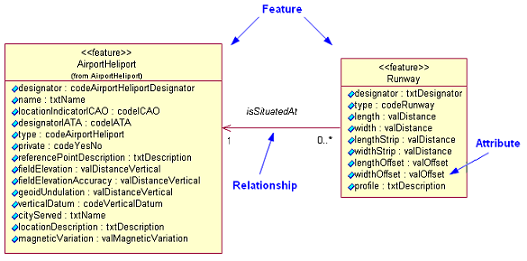
\includegraphics[scale=0.5]{aixmUML.png}
\end{center}
\caption{UML diagram highlighting some features of the AIXM conceptual model.\cite{aixm}}
\label{fig:aixm}
\end{figure}

\newpage

\subsection{Publish/Subscribe Architecture}
\label{sec:bg_pubsub}

\begin{figure}
\begin{center}
\def\svgwidth{\columnwidth}
\input{broker.pdf_tex}
\end{center}
\caption{Publish/Subscribe Architecture with Broker}
\label{fig:pubsub}
\end{figure}

Publish-subscribe is a messaging architecture that allows decoupling between the \emph{producers} and the \emph{consumers} of \emph{messages}. Messages are categorised into \emph{topics}; producers publish messages on a given topic without requiring knowledge of which (if any) subscribers the topic has, and consumers subscribe to a given topic with no knowledge of which (if any) producers are publishing messages with that topic.

This architecture is generally implemented using a \emph{broker}, which exists as middleware between the producers and consumers. Producers send messages on a given topic to the broker, which then decides which consumers the messages should be forwarded to. Consumers subscribe via the broker to topics they’re interested in, and the broker forwards relevant messages to them. This architecture has a number of benefits, including providing loose coupling between producers and consumers (since they need no knowledge of each other to make use of this architecture) and facilitating scalability by supporting arbitrary numbers of producers and consumers for any given topic.

In Java, brokers typically implement the Java Message Service (JMS) API provided by Java Enterprise Edition, which offers a consistent interface for communicating with many different message broker implementations.

\subsection{Web Services Notification}
\label{sec:bg_wsn}

Web services notification (or WSN) is a set of specifications created by OASIS that defines the interactions between web services, using notifications, which can form the basis of a publish/subscribe architecture built using web services. They provide a standardized way to communicate with and between web services, without having prior information about them. It includes facilities for detailed subscription, where those wishing to consume information can register with a web service along with details about the type of information they wish to receive. WSN was designed to revolve around these subscription details known as ``topics'' and use them to filter down subscriptions, allowing for large scale usage of the publish/subscribe architecture without unwanted message overload.

WSN covers a family of smaller specifications including WS-Base Notifications, WS-Brokered Notification and WS-Topics. WS-Base Notifications is a specification of the simple producer/consumer relationship, consumers send out subscription requests to the producers, specifying the subset of messages produced by that producer which it wishes to receive. The request also contains a reference to the consumer itself, so the producer knows where to send the messages.

WS-Brokered Notification works in a similar manner to WS-Base, but introduces a middleman between the message publishers and the message subscribers known as the broker. The broker is designed to decouple the connection between producers and consumers and allows for advanced messaging features such as demand-based publishing, load-balancing and publication of messages from entities which are not themselves web service providers.

WS-Topics is a specification which defines a method for categorising subscriptions into ``topics''. This specification is designed to work in conjunction with WS-Base or WS-Brokered and contains various methods for defining groups of subscriptions.

\subsection{Web Services Description Language}
\label{sec:bg_wsdl}

The Web Services Description Language (or WSDL) is an XML based language for describing the interfaces and functionality of a web service. A WSDL file provides a machine readable description of a web service's interface, including the function calls, parameters they expect and return values.\\
Typically, it is used in combination with SOAP to provide a web service, where a client program will read the WSDL, to determine the functions available, and then use SOAP to call them.

\subsection{JAXB and DOM Parsing}
\label{sec:bg_parsing}

JAXB, or ``Java Architecture for XML Binding'', is a tool used to marshal Java objects into XML and unmarshal XML into Java objects. It can be used as an alternative to standard XML parsers, taking complicated schema and converting XML created from them into usable Java objects. Use of JAXB was explored towards the end of the project for use in spatial filtering. It was intended to use JAXB to parse XML filters of the OpenGIS standard in order to create filters within our system, however, implementing JAXB proved beyond the scope of the project in terms of time, given the nature of the system as a proof of concept piece with a strict time constraint. Instead, a more commonly used XML parsing method known as ``Document Object Model'' or DOM parsing was settled on.

DOM parsing is one of the two most commonly used XML parsing methods, the other being SAX parsing. A DOM parser works by loading the entirety of an XML document into memory, modelling it as a tree to allow it to be easily traversed. The tree is traversed node by node to obtain the required information, in this case known tags within the OpenGIS standard for use in spatial filtering. This method of parsing generally has quite a large overhead when parsing large XML files, due to the fact it needs to parse the entire file.

\subsection{XML Catalogues}
\label{sec:bg_catalogues}

XML files contain references to external XML resources such as schema files and WSDL files. When referencing a large number of external files, events such as network outages and slow connections can cause major issues for a service and its performance. Another problem which can occur when referencing external resources is relative URLs being used to address them. Relative URLs limit the service using them to the context in which it was created, as launching it from any other location will not work.

A solution to these problems is creating an XML catalogue, which allows you to store these files locally and instruct your service to use these local references when its external counterpart is requested. The catalogue maps between these two versions of the same resource.

\subsection{JIRA Issue Tracking}
\label{sec:bg_jira}

Issue trackers are systems which maintains lists of issues in an ongoing project, with the ability to assign these issues to specific group members, report bugs while working and connect solved issues to source control commits which fix them. Issues can also be broken into sub-tasks, prioritised and categorised to improve efficiency. For example, many issues were recorded after each sprint meeting, these included work for the next sprint, work for near future sprints and overall project goals. These issue reports were categorised according to the sprint which they were to be completed in. When every issue attached to a sprint was marked as solved, a sprint was considered complete in terms of work.

As the customer is a company which regularly works on projects of a much greater scale than that of the AES system, they possess a number of professional tools for organisation and issue tracking. One of these is JIRA, an issue tracker created by Atlassian designed to work with the chosen cycle of creating user stories and acceptance criteria with the customer and assigning these stories to team members after each sprint meeting. As JIRA is a professional piece of software which normally requires a monthly fee for usage, it had to be accessed via the server running it licensed to the customer through their VPN. By using the tools in use by the customer, they were able to easily keep track of progress and make comments on submissions to the service.

\subsection{ActiveMQ}
\label{sec:bg_activemq}

Apache ActiveMQ is an open source message queue service which communicates using the Java Message Service (JMS). It contains a number of features deemed useful to the project including subscription management and filtering. The filtering itself is through objects known as selectors, which use the SQL 92 syntax to filter messages. SQL 92 is a fairly barebones SQL syntax, which features basic arithmetic operators (addition, subtraction, multiplication, division and modulo), enough for the requirements set out by the customer of temporal filtering and spatial filtering using GPS co-ordinates.

\subsection{Git and GitHub}
\label{sec:bg_git}

Git is a distributed version control system, which allows multiple people to work on a single project at the same time, without necessitating the use of a shared network, as well as tracking document history, affording reversions or rollbacks to previous versions. Some form of source control is essential for effective collaboration between programmers and greatly aides coordination and communication.

GitHub is a Git repository hosting service, which also offers other features that aide collaborative coding, such as issue tracking and task assignment.

\subsection{Travis CI}
\label{sec:bg_travis}

Travis CI is a free, hosted, continuous integration platform that is used to automatically build and test projects hosted on GitHub. It automatically detects when a commit has been pushed to a linked GitHub repository and attempts to build all branches and run tests. It can then be set up to show the results of this in the GitHub readme or to notify the developer in some other way, such as by emailing the results.

This practice of continuous integration allows developers to detect problems quickly. This also makes fixing them easier, as less back tracking is required to identify when and where an issue occurred, reducing the number of large scale revisions required. It also means they can assure the software will run on a variety of computer set-ups, without time consuming manual testing.

\subsection{Cucumber}
\label{sec:bg_cucumber}

Cucumber is a testing suite that runs behaviour-driven development style acceptance tests, i.e., tests written to check if the requirements of a specification are met by the code. These focus on testing behaviours, i.e. the action the code is supposed to perform, where each test goal is independent of the code’s structure, rather than an approach like unit testing, that tests individual units of code.
A single Cucumber test consists of a plain text feature definition, written in plain English, and corresponding step definitions, that is, the code that actually tests the feature.

A feature definition describes a single behaviour the code is supposed to be able to perform (such as ``Feature: Filter NOTAMs by time'') and then outlines one or many scenarios: sets of conditions that test a facet of the behaviour. These describe initial conditions, steps that are then carried out, and what the results of performing those steps (with those initial conditions) should be. These are specified with the keywords ``Given, When, Then'', i.e., given a set of initials conditions, when something happens, then the program should do something (with the ability to have multiple steps with the keyword And).

For each feature, there is then a set of corresponding step definitions, that is, code to test the feature, in the form of a subroutine for each step (e.g. there will be a single subroutine for ``Given a broker is running'', which will check that a broker is running and, if not, launch one). Depending on the keyword, these should either set up the initial conditions (in the case of Given or a following And), perform a particular action (in the case of When or a following And), or assert that particular conditions are true (in the case of Then or a following And). If all conditions are satisfied, the test passes, otherwise it fails.

\subsection{JSON}
\label{sec:bg_json}

JSON (or JavaScript Object Notation) is a human readable data interchange format and an alternative to XML. It transmits data objects consisting of attribute-value pairs and is primarily used for server-web application communication. One of its primary advantages is its relative concision and lack of redundancy when compared to XML.

\subsection{SOAP}
\label{sec:bg_soap}

SOAP (or, originally, Simple Object Access Protocol) is a platform independent protocol for exchanging information between web services, based on XML, and is dependant on other application layer protocols for message transmission (typically HTTP but other transport protocols are supported as well).

\subsection{Netcat}
\label{sec:bg_netcat}

Netcat is a utility to read from and write across network connections using TCP or UDP. It is designed so that it can easily and reliably be used as a back-end tool, so it can be used by other programs. It is frequently referred to as the `Swiss army knife' of networking tool because of its wide array of features, such as port scanning and a large number of network debugging and investigation tools.

\subsection{cURL}
\label{sec:bg_curl}

cURL is both a library and command line tool for sending and retrieving data using a wide variety of protocols (such as HTTP, FTP, SCP, POP3, etc.). It is very portable, working on a wide variety of platforms, and bindings are available for a large number of programming languages.

\subsection{Web Feature Service}
\label{sec:bg_wfs}

\newpage

\section{Planning and Organisation}
\label{sec:planning}

\subsection{Software Development Methodology}
\label{sec:plan_software_development_methodology}

The project was built using the Agile software development practices of Scrum, with each sprint following a similar structure. Every other week, the team would meet at Snowflake Software's main offices. First, the customer came up with ideas for features which could be worked on in the following sprint. Next, user stories based on these features were created, dividing up the requirements of each feature and helping to create acceptance criteria which would come together to prove acceptance that the feature was successfully implemented.

\subsubsection{Meetings} 

At the beginning of each sprint, a sprint meeting was held to both close the previous sprint and prepare for the following one. First, features implemented in the previous sprint were demonstrated to the customer, allowing them to track the progress of the project and decide if the feature had been successfully implemented. In the event that the customer was not satisfied with the work done in the sprint, the user stories were kept in the backlog for the following sprint. Otherwise, the customer discussed future features to be implemented and broke the feature up into user stories to be added to the backlog.

Meetings also regularly featured exercises to identify issues and find solutions to problems faced by the group over the previous sprint. Before moving onto work that needed to be done for the following sprint, each group member and the customer filled in a table of three columns on a whiteboard. These columns listed points members felt happy about in terms of project progression, points unsure about and points the members felt required discussion. This list was then prioritised and discussed in order, finding solutions for problems such as group dynamic issues and ensuring the practises members agreed were going well were maintained. These exercises not only created a more open forum for members of the group to start discussions about things they might otherwise be uncomfortable discussing, but allowed the customer to maintain awareness of aspects of the project which were working well.

\subsubsection{Tools}

Various software was used to aide this process, including JIRA (access to which was provided by the client) and Cucumber. JIRA is a tracker that manages user stories and their corresponding acceptance criteria as per each feature. User stories within JIRA are stored in the standardised \emph{``As a, I want, So that''} format, with their acceptance criteria written as \emph{``Given, When, Then''}. This format is also used by Cucumber for acceptance tests. Team members on JIRA can choose what user stories to complete or they can be assigned.

Early on in the project, the group was given access to Jira on Snowflake's private servers. This allowed control over the backlog to be maintained and a record of what had been completed to be kept. However over the course of the project, the number of steps required to connect to the Snowflake VPN and access Jira, as well as the difficulties arising from never having used the service before, it was decided that keeping track of the project would be better done through GitHub, which was already being used as a code repository. The issue tracking features within GitHub replaced Jira's extensive features (the majority of which far surpassed the requirements of a small project such as this) and all tasks became issues, still using the standard user story format.

\subsection{Skills Audit}
\label{sec:plan_skills_audit}
To maximise the efficiency of the team and to minimise the amount of time which needed to be spent learning new skills for the project, it was necessary to assign tasks according to relevant skills and experience. In order to do this it was necessary to produce a skills audit (shown below) and divide tasks according to it.

\begin{table}[h]
\begin{tabular}{|l|l|}
\hline
\emph{Team Member} & \emph{Relevant Skills}                           \\ \hline
Andrew Sullivan    & Java, Python, JUnit                              \\ \hline
Charles Sherman    & Java, WSDLs, SOAP-UI, JUnit, Cucumber, SCRUM     \\ \hline
Peter Prince       & Java, Python, JUnit                              \\ \hline
James Robinson     & Java, Maven, Git, JIRA, Travis, Cucumber, JUnit  \\ \hline
\end{tabular}
\end{table}

During each sprint meeting the work for the following sprint was decided upon, followed by a meeting in labs to break down the sprint work further and assign each key area to a team member according to their relevant skills. Due to the nature of the project, a lot of early work on the project was not easily divisible, so a system of a single team member coding as the rest of the team researched and provided support, was used.

\subsection{Risk Analysis}
\label{sec:plan_risk_analysis}

Assigned to Charles

\subsection{Customer Relations}
\label{sec:plan_customer_relations}

The project customer was Snowflake Software, a Southampton-based company specialising in open data exchange solutions. Over the course of the project, regular sprint meetings were held with a number of Snowflake employees, including one of the CEOs, Ian Painter; the chief technology officer, Eddie Curtis; the professional services director, Alex Brooker; head of software development, Adrian McKenzie (who acted as the main liaison with the company), as well as a number of members of their development team who were present in the final presentation to the company of the finished product. Communication with Adrian was done through both emails and the fortnightly Scrum meetings.

\subsection{Git workflow}
\label{sec:plan_git_workflow}

Assigned to James

\subsection{Testing Methodology}
\label{sec:plan_testing_methodology}

Behavioural-driven development style acceptance testing was used, using Cucumber to express the acceptance criteria for each story, allowing them to be converted into automated acceptance tests which could be run using JUnit. The scenarios were written such that the implementation of the feature can change without the file needing to be rewritten. For each story, when all acceptance tests passed within JUnit, the user story was removed from the backlog. This type of testing keeps testing focused on user stories, testing features rather than abstract units of code, better ensuring that the code satisfies the client's requirements, rather than some abstract measure of performance.

Continuous integration was also used, utilizing Travis CI. This helps to ensure new code doesn't break old tests, ensures the software can run on a variety of computer set-ups, and allows problems to be detected more quickly and fixed with less backtracking.


\newpage

\section{Implementation}
\label{sec:implementation}

Due to the exploratory nature of the project, there was a lot of work that went into the project that wasn't present in the end result. The team worked using SCRUM and completed five sprints. In the implementation, each sprint is discussed individually to show the alternatives explored and to show the work that didn't make it to the final prototype.

\subsection{Sprint 1}
\label{sec:impl_sprint_1}

At the start of the project, the team had a meeting with Snowflake, were introduced to the project and discussed the scope, requirements and overall goals of the project. Snowflake described the vision of the project, the goal set was: ``To demonstrate the feasibility of using Publish/Subscribe to communicate relevant NOTAMs to flight planners''. This also had to be implemented using either the WS-Notification standard or WS-Events, as these are the most used standards in the industry.

\subsubsection{Sprint Goals}

For the first sprint, the goal was to have a basic push notification system running that could publish and receive an XML. As well as this, the development environment and tools for the project had to be set up.

The project was written in Java because of the familiarity the team already had with it. The team worked in the IDE Eclipse, and used the build system Maven to handle library dependencies, as it has automatic dependency resolution and plugins for code generation. For version control the team used GitHub.

For the first sprint, there was only a single user story to implement. Jira\ref{JIRA} was used to manage the user stories and to allocate the work, however there were problems using it.

\userstory{Basic Push Notification}{flight planner}{to be notified if there is a change to my destination airport for my planned flight.}{I can change my plan in response to events involving airspaces and runways on my route.}

To implement the user story required setting up Apache ActiveMQ\ref{activeMQ} and implementing a method of providing a message to the broker and a way of displaying the message so tests could be written to see that it was received correctly.

\subsubsection{Work Allocation}

As the sprint goal was very simple, it was difficult to separate the work between team members. The majority of the coding work was done by James, whilst everyone else in the group assisted by researching the possible tools that could be used. This was, in effect, an extension of pair-programming, where two people working on a single machine take turns in programming while the other critiques and checks for mistakes.

Once a solution that worked has been found, James presented the code to everyone else so that the group understood the chosen implementation and the motives behind it.

Apart from programming, James also helped to set up Maven on the team member's machines so that they could also work on the code. Charles Sherman set up the GitHub repository to store the code for the project and Peter Prince set up the team's project on Jira.

\subsubsection{Implementation}

After working on a basic implementation of ActiveMQ and exploring the documentation available online, it became obvious that it contained no implementation of WS-Notification and the page within its online documentation which was supposed to detail its implementation was a dead link. One of the requirements stated by the customer was the inclusion of WS-Notification and whilst this was a soft requirement, meaning that it's inclusion could be forgone if sufficient justification was given, the project was in an early enough stage at this point in development that it was worth exploring other alternatives; alternatives such as developing a WS-Notification implementation from scratch using CXF.

Apache CXF is an open source framework for producing web services, and after ActiveMQ was deemed unusable, research began into using CXF. Work started by creating a WS-Notification implementation within CXF. Progress in this was slowed significantly by documentation for the framework being extremely limited. Whilst creating this implementation, it was discovered that an implementation already existed, undocumented, within Apache CXF. Through experimentation and knowledge gained from attempting to build a bespoke implementation, a basic demo was produced, subscribing a consumer to a preallocated topic and sending out a message through the subscription.

\subsubsection{Review}

At the end of the first sprint, the first user story had been completed and the development environment set up for all the team members. Eclipse with Maven was working on everyone's machines and using GitHub, the code that had been written was shared, so that in future sprints everyone would be able to work on the code.

The major issue in this sprint was the bottleneck caused by the coding. It was impossible to divide up the programming work between group members, which made it difficult to progress through the work quickly and to keep everyone informed about the work. Although it was inefficient, by having one team member write the code whilst everyone else researched, this did mean that everyone was at least familiar with the project so that they would be able to work efficiently in future sprints. At the end of the sprint, the team had a meeting without the customer, where the code was reviewed, so that everyone understood it and could work on it in the future sprints.

There were issues with writing the user stories to Jira. Peter and Andrew were the only people who could access the online service due to issues with the web plugin on other team member's machines. This made the point of assigning work to group members on Jira useless, as people couldn't see what work they had been given. This issue was solved in the next sprint where Jira was replaced with GitHub issue tracking.

\subsection{Sprint 2}
\label{sec:impl_sprint_2}

\subsubsection{Sprint Goals}

In the second sprint, the goals set were to expand on the work completed in the first sprint. At the end of the first sprint, a producer, broker and consumer had been written, all with hard-coded values for the subscription information. The target for the end of the second sprint was to have a consumer that subscribed with configurable topics, and to have multiple consumers listening to a broker. It was also important to develop tests to demonstrate to the customer that the software was working, and for the team to manage bugs that arose in development.

\begin{table}
    \begin{tabular}{|l|l|l|l|}
    \hline
    \emph{Origin}         & \emph{Destination}    & \emph{Route}                 & \emph{Consumers} \\ \hline
    One Hard-Coded & None           & None                  & One       \\ \hline
    Configurable   & One Hard-Coded & One Hard-Coded        & Two       \\ \hline
    ~              & Configurable   & Multiple Hard-Coded   & Multiple  \\ \hline
    ~              & ~              & Multiple Configurable & ~         \\ \hline
    \end{tabular}
\caption{Sprint 2 Table}
\label{tab:sprint2}
\end{table}

During the second sprint planning meeting a table of requirements was made with Snowflake. The table split the tasks into layers that had to be implemented row by row, but within each row the columns were independent and could therefore be completed in any order. At the start of the sprint, the top row of the table had already been completed and the target for the end of the sprint was to have the lowest row from each column implemented. The process works by filling out each layer of the table, one at a time to make sure features could be implemented in feasible steps.

\userstory{Notification Filtering By Airport}{flight planner}{to be notified if there is a change to airports I'm interested in for my planned flight.}{I can change my plan in response to events involving airspaces and runways on my route.}

\subsubsection{Work Allocation}

Peter and James worked on rewriting the code so that multiple subscriptions were possible and could be configured by command line arguments. Charles was assigned writing tests for the system using Cucumber.

\subsubsection{Implementation}

In practice it was found that the jump from hard coded values to fully configurable parameters was trivial. However, creating tests for the code was not as simple as hoped. A set of Cucumber tests was created to check that a NOTAM could be sent from a producer, to a broker and out to a set of consumers. There were issues with starting multiple processes up and having time-outs to check if a NOTAM had been received.

\subsubsection{Review}

It was at this point, after producing a large number of user stories for this sprint, that the decision to cease using JIRA for issue tracking was made. At this point in the project, the group getting bogged down by the many unused pages and tools of JIRA which served no purpose to the small project, so it was decided to switch entirely to GitHub's issue tracker which was already being used in a minimal capacity. While JIRA initially proved useful early on in the project, having to install and use the VPN software on every computer that needed access to the tools meant the issue tracker provided by the source repository (GitHub) ended up being temporarily used as a middleman. Shortly after it was decided that this was not an efficient use of time, the group debated leaving JIRA in favour of fully committing to GitHub. While a number of tools offered by JIRA did not exist in GitHub's issue tracker, this often worked against JIRA, as it contained a large array of tools not useful for a small scale project such as this, which often got in the way. As GitHub was already being used as the source repository, bringing issue tracking and source control into one place seemed like the most efficient thing to do.

Having tests for the system would have been useful but they only worked on certain team member's machines. This made the tests counterproductive as they would sometimes give the impression that the system was working when it would only work on one machine, in a specific set of circumstances. There were also issues with setting up and pulling down services, such as the notification broker, between tests. Additionally since the tests ran every time the code was compiled this slowed the development process considerably when long timeouts for the tests had to be included. In sprint 3, the tests were moved to Travis CI, which solved all these problems.

\subsection{Sprint 3}
\label{sec:impl_sprint_3}

\subsubsection{Sprint Goals}

The main focus of sprint 3 was to research the extent of JBoss A-MQ's filtering capabilities, to access its viability for use in the project. Through research in the previous sprint, the prominence of JBoss as a message queue used industrially had become apparent. Research done by Snowflake themselves also suggested that it would be useful for the project. The subject of testing was also brought up, and the implementation of a continuous integration system was decided upon to streamline the implementation of changes to the project. Early on in the sprint, Jenkins was implemented and set up to run tests continuously on the latest version of the project, updating the project's GitHub page with the outcome of the latest tests.

It was in sprint 3, after the progress made up to that point was shown in the sprint meeting, that another representative of Snowflake expressed the importance of spatial filtering over temporal filtering. The utility of spatial filtering is obvious in the case of flight planning, a flight planner simply defining the start and end point of the journey and then receiving all messages relevant to that geographical space would save considerable time when compared to the alternative of manually subscribing to airspaces and airports which are within range. Temporal filtering would allow a consumer to only receive NOTAMs that are in effect for the duration of their flight, dramatically reducing the number of irrelevant NOTAMs being sent.

In order to perform spatial filtering, latitude and longitude data for every airspace and airfield would be required, as NOTAMs lack information at this level of detail. The information required for temporal filtering is featured in each NOTAM, and only conversion to a usable timestamp format was required.

Additionally, one of the team's main desires was to fix the problems with the Cucumber tests. The tests were slow and would only work on certain machines; a goal was set for the team to find a way to remedy this issue. It was decided that the tests should be moved to a continuous integration server and to not run the tests every time the code was compiled.

\subsubsection{Work Allocation}

Charles continued working on the Cucumber tests, writing more case scenarios and fixing bugs in the old tests. He also set up the GitHub repository to work with the continuous integration service on Travis. James was assigned changing the system over to JBoss. In the middle of the sprint it became apparent that JBoss wouldn't be able to meet the requirements, so James then started to work on a JMS system. Pete looked into temporal and spatial filtering and was set the task of writing a basic test scenario to check basic filters based on GPS co-ordinates could be produced.

\subsubsection{Implementation}

With these two filtering types being the goal of the sprint, work was split into exploring documentation for implementation instructions and information regarding filtering, in JBoss A-MQ. After a week of investigation, it became apparent that JBoss did not have the capabilities to fulfil the requirements of the product, due to its extremely limited filtering implementation. JBoss filtering is restricted exclusively to simple strings, comparing the contents of each message with a given filter and sending based on its presence. This left two options: either forking A-MQ and modifying it to support the required features, or dropping it in favour of a message queue which does fulfil those requirements. Basing the decision on the scope of the project and limited remaining time to complete it, it was decided to abandon A-MQ. As it was early in the sprint and the outcome of the decision would dramatically affect the outcome of the sprint, the customer was notified of the decision, to ensure it was satisfactory to them.

Once the decision had been made to use JMS, a filtering proof of concept was required to justify the change. Using JMS Selectors to filter based on dummy GPS co-ordinates randomly assigned to each NOTAM, a basic implementation of spatial filtering was created.

Moving the Cucumber tests to Travis CI was done with little difficulty. As the team was already using Maven for the project, the only work that was required was in creating a configuration file to call the relevant tests. The issues with startup and teardown with the Cucumber tests were fixed by rewriting the consumer and producer code so that they could be run in a single process rather than in multiple ones. When the tests were moved to running on Travis CI rather whenever the code was compiled, they were instead run every time a commit or a merge request was made, which worked well with the Git workflow of the group.

\subsubsection{Review}

In this sprint, a major shift was made from JBoss A-MQ to a JMS-based service. This change required a large amount of work to complete, but allowed work to start on filtering. Basic spatial filtering was created and filtered NOTAMs based on dummy GPS co-ordinates, requiring NOTAM enrichment to complete this feature.

Cucumber tests easily made the transition on Travis CI and improved consistency with the existing Git workflow.

\subsection{Sprint 4}
\label{sec:impl_sprint_4}

The forth sprint meeting consisted of bringing up to speed members of Snowflake in attendance who had not been notified about JBoss A-MQ. As well as the product owner, Eddie, and the scrum master, Adrian, Alexis Brooker also attended, and after discussing the need for GPS locations in order to perform spatial filtering, Alexis provided access to a HTTP-GET web feature service (WFS), which returns latitude and longitude locations for all European airfields. Ideally, calling this service would be implemented into AES itself, however given the time remaining on the project and the status of the product as a proof of concept, it was elected to simply retrieve data for all airfields and hard-code them into the system for use in spatial queries, knowing that the system could easily be modified to directly call the service and utilise the data if more time was spent on it.

\subsubsection{Sprint Goals}

After JBoss A-MQ proved to be a dead end, a new system structure was decided on, with only the consumer side using WS-Notifications to communicate. All remaining communication between brokers and producers was changed to rely on JMS, with converters between WS-Notification topics and JMS filters becoming a primary focus for the sprint.

To implement the goals of spatial and temporal filtering, NOTAM enrichment was required.


\subsubsection{Work Allocation}

For this sprint, Charles was assigned the task of building more elaborate temporal filtering; in parallel to this, Peter worked on spatial filtering, James was tasked with implementing the WS-Notifications standard into the system and Andrew created an XML document which contained a subset of all airport locations, narrowing them to just European aerodromes. Due to the large number of global aerodromes, it was necessary to reduce this just to relevant locations in the interest of parsing time.

\subsubsection{Implementation}

Temporal filtering was implemented by parsing the NOTAM XML and converting the timestamps in the data to a Unix time stamp format. The time stamp measures the time in milliseconds, so it is possible to directly compare the times using inequality operators. The code allows a consumer to subscribe to topics after a given time, or within a time period.

The selectors used for filtering are based on SQL 92, which features only simple arithmetic operators. In order to create a proper bounding box which covered a plane route, more operators were required (such as square roots, which are not included). As a result, spatial filtering's implementation was simplified to an axis-aligned bounding box. This type of spatial filtering required simply greater than and less than operators to perform.

To produce the subset XML document, a bounding box was placed over Europe and submitted to the Global Aerodromes service, all aerodromes within the given bounding box were retrieved.

\subsubsection{Review}

All required features of JMS (selectors and subscriptions) were successfully added, however a functioning implementation of the WS-Notification standard could not be created. This goal was moved to the final sprint as a primary focus.

\subsection{Sprint 5}
\label{sec:impl_sprint_5}

\subsubsection{Sprint Goals}

The goal for the final sprint was to produce a complete minimal viable product for the product owner. This involved finishing our WS-Notification implementation, packaging the application as a WAR for deployment on Tomcat, building a WSDL for the web service, making a barebones client to demonstrate the service's functionality, and implementing basic OpenGIS filtering support. We also planned to replace our DOM parsers with JAXB in order to make it easier to implement the OpenGIS filtering support.

\subsubsection{Work Allocation}

\begin{tabular}{l|l}
  \emph{Task} & \emph{Assignee(s)} \\ \hline
  JAX-WS code generation using CXF Maven plugin & James \\
  WSDL for our WS-Notification implementation & James, Charles \\
  WAR generation using Maven & Charles \\
  Tomcat setup and WAR deployment & Charles \\
  Mapping from OpenGIS filters to JMS selectors & Peter \\
  Mock client implementation using NetCat and cURL & Peter \\
  Barebones client implementation using JAX-WS & James \\
  NOTAM enrichment & Peter, Andrew \\
  Parsing the Snowflake GlobalAerodromes WFS & Andrew \\
\end{tabular}

\subsubsection{Implementation}

We used the Apache CXF JAX-WS codegen plugin for Maven to build class stubs from the WSN WSDLs. Unfortunately the WSDLs provided by Oasis do not specify any endpoints, and so we created our own based on a subset of the WSN WSDL included with the Apache CXF implementation of WSN.

A mock client for the system was implemented using NetCat and cURL - NetCat took the place of the WSN consumer, listening on port 80 and simply printing out all received data to standard output, and cURL was used to send a subscription request to the WSN broker. Unfortunately we were unable to determine the correct format for the subscription request, so we ditched the barebones client implementation and created a new implementation using CXF, based on the WSDL for our web service.

We originally planned to switch to JAXB for our XML parsing needs during this sprint, but there were so many naming conflicts in the generated code for the XML schemata that it was easier to just manually write DOM parsers instead. After consulting with Snowflake we discovered that they too attempted to use JAXB but abandoned it due to the same issue.

\subsubsection{Review}

We were able to complete all of our goals for this sprint, and produced two projects - the AES service itself, consisting of our producer and WS-Notification broker implementation, and a separate project containing an example consumer.

\subsection{Final Meeting}
\label{sec:impl_final_meeting}

The final meeting consisted of the group demoing and explaining the finished project (i.e. the results of sprint 5), not just to the usual customer representatives, but to a large number of other Snowflake employees that had no previous involvement with or knowledge of the project (including the CEO and a number of both technical and non technical roles). Once the demo was concluded, the group fielded questions, both from the original customer representatives about the progress in the last sprint, and from those new to the project about the project as a whole.

The demo consisted of a single producer and a single broker running throughout, with consumers each subscribing to individual topics; this demonstrated that the software can deal with multiple clients and demonstrated that it was actually performing filtering based on topics (as opposed to a precooked demo that could be used to mislead). Once the demo was complete (and after a member of Snowflake requested a demonstration of a topic of their own choosing), the general architecture of the system was explained (as seen in figure 3).

Since it was the final meeting, the typical sprint review was omitted, since the project was completed and it was no longer needed to guide the direction of the next sprint.  Instead, once the initial meeting with Snowflake at large was concluded, there was a discussion of the project as a whole with just the original client representatives (Adrian and Eddie). Here the total project progress was discussed, as well as how the work would be used and developed further (by Snowflake) in the future. 



\section{Final System Overview}
\label{sec:final_system}

\begin{figure}
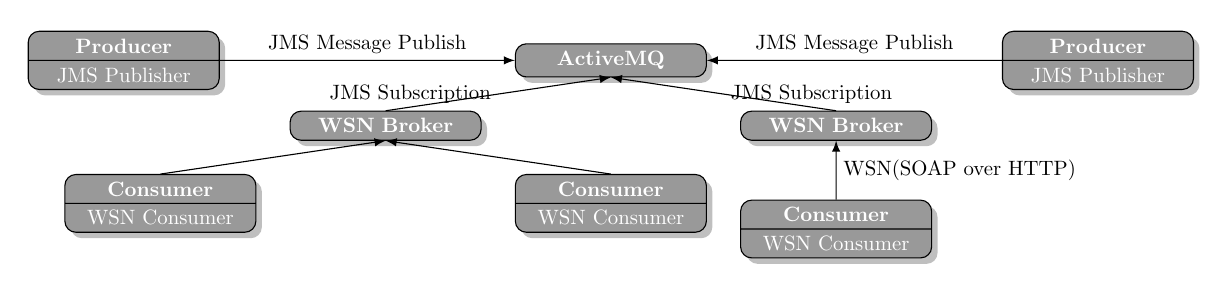
\begin{tikzpicture}[scale=0.75, every node/.style={transform shape}, node distance=2cm]
     \node (Producer1) [abstract, rectangle split, rectangle split parts=2]
        {
            \textbf{Producer}
            \nodepart{second}JMS Publisher
        };

    \node (ActiveMQ) [abstract, rectangle split, rectangle split parts=1, right=5cm of Producer1]
        {
            \textbf{ActiveMQ}
            
        };

    \node (Producer2) [abstract, rectangle split, rectangle split parts=2, right=5cm of ActiveMQ]
    {
        \textbf{Producer}
        \nodepart{second}JMS Publisher
    };

    \node (WSN Broker1) [abstract, rectangle split, rectangle split parts=1, below left=0.8cm of ActiveMQ]
        {
            \textbf{WSN Broker}
            
        };

    \node (WSN Broker2) [abstract, rectangle split, rectangle split parts=1, below right=0.8cm of ActiveMQ]
        {
            \textbf{WSN Broker}
            
        };

    \node (Consumer) [abstract, rectangle split, rectangle split parts=2, below right=0.8cm of WSN Broker1]
    {
        \textbf{Consumer}
        \nodepart{second}WSN Consumer
    };

    \node (Consumer1) [abstract, rectangle split, rectangle split parts=2, below left=0.8cm of WSN Broker1]
    {
        \textbf{Consumer}
        \nodepart{second}WSN Consumer
    };

    \node (Consumer2) [abstract, rectangle split, rectangle split parts=2, below=1cm of WSN Broker2]
    {
        \textbf{Consumer}
        \nodepart{second}WSN Consumer
    };

    \draw[-latex] (Producer1.east) -- (ActiveMQ.west) node[midway,above] {JMS Message Publish};
    \draw[-latex] (Producer2.west) -- (ActiveMQ.east) node[midway,above] {JMS Message Publish};
    \draw[-latex] (WSN Broker1.north) -- (ActiveMQ.south) node[midway,left] {JMS Subscription};
    \draw[-latex] (WSN Broker2.north) -- (ActiveMQ.south) node[midway,right] {JMS Subscription};
    \draw[-latex] (Consumer.north) -- (WSN Broker1.south) node[midway,right] {};
    \draw[-latex] (Consumer1.north) -- (WSN Broker1.south) node[midway,right] {};
    \draw[-latex] (Consumer2.north) -- (WSN Broker2.south) node[midway,right] {WSN(SOAP over HTTP)};

\end{tikzpicture}
\caption{System overview}
\label{fig:system_overview}
\end{figure}

The completed system consists of two parts: a producer, which parses NOTAM data and publishes it to a JMS broker (ActiveMQ, in our project), and a basic WS-BrokeredNotification implementation that allows consumers to retrieve messages from this JMS broker via the WS-Notification protocol. An block diagram giving an overview of this system is provided in figure~\ref{fig:system_overview}.

The system was designed with scalability in mind, since it needed to be able to handle a large volume of NOTAM traffic, and a potentially large number of consumers. For this reason, an arbitrary number of producers and an arbitrary number of WS-Notification brokers are supported, with each broker servicing multiple consumers. The limiting factor in this setup is the number of simultaneous connections that the JMS broker itself is able to service. Since ActiveMQ already has robust support for clustering, this was deemed to be a non-issue.

Although the consumer was out of this project's scope, we still produced a basic implementation in order to demonstrate the system's functionality. A class diagram for this separate project is given in figure X. Note that this project does not directly reference any of the classes from our main project; instead, it uses the published WSDL for our service, along with JAX-WS, to connect to the service.

\section{Critical Evaluation}
\label{sec:critical_evaluation}

In order to properly judge the success of a project such as this, it is important to compare the finished product to the requirements and goals set out initially. This can be somewhat difficult when Scrum is used to manage the project, given how goals and requirements are subject to change each sprint. Thankfully, the overall scope of the project only received minor alterations, so almost all of the requirements initially set out by the customer remain relevant to the final product. Every requirement was met, with come concessions made with respect to features such as complex spatial filtering in the interest of time and given the fact that the product is a proof of concept for future works rather than a product to be used by flight planners.

\subsection{Git workflow}
\label{sec:eval_git_workflow}

Assigned to James

After we switched to the new workflow, this worked pretty well

\subsection{Project management}
\label{sec:eval_project_management}

Using GitHub issues worked well, but didn't provide us with things like burndown charts, etc. that traditional agile project management tools provide

\subsection{Customer feedback}
\label{sec:eval_customer_feedback}

In addition to the feedback given in sprint planning meetings throughout the project, and the feedback given in the final meeting, at the group's request, Snowflake sent an email with some feedback and reflections on the project performance and outcome, as shown in the appendix.

The feedback was mostly positive, particularly focusing on the exploratory goals of the project, i.e., the successful evaluation of the usefulness of a large number of technologies to the project (the as a whole, including the continued development by Snowflake, rather than just limited to the scope of the GDP work). Even though it was determined that most of those technologies were wanting, it was not wasted effort, since had it not been done, Snowflake would have had to have gone through the same exploratory process.

\blockquote{...good outcome for Snowflake Software; they answered some of our key questions and provided a solid foundation to commence our Pub-Sub product development in 2015... Reaching firm conclusions about the relative merits of the technologies you assessed represents a real achievement.}

Their main criticism was the one sidedness of the sprint planning meetings and of the final meeting, where a large proportion of the speaking and demonstration was done by James.

\section{Conclusions}
\label{sec:conclusions}

\newpage

\section{Future Work}
\label{sec:future_work}

\subsection{Performance/Scalability Testing}
\label{sec:future_testing}
%Performance/scalability testing (using Amazon EC2 and/or Elastic Beanstalk for example)
Assigned to James

\subsection{IATA Designators and ICAO Location Indicators}
\label{sec:future_designators}

Global Aerodromes is a service provided by Snowflake which allowed our system to map from aerodromes referenced in NOTAMs to GPS co-ordinates, a feature required in order to perform spatial filtering. Within the AIXM specification for NOTAMs, both IATA (International Air Transport Assocation) designators and ICAO (International Civil Aviation Organisation) location indicators are specified. Both of these designating IDs are used by Global Aerodromes and the AES service we produced made use of just IATA designators to pair NOTAMs to GPS co-ordinates. This caused an issue due to a fraction of the aerodromes listed by the Global Aerodromes service do not contain a value for this identifier. A possible future extension would be to add a contingency for this occurrence and include support for ICAO location indicators as well, to maximise the chance that every NOTAM's aerodrome is matched to a location for filtering.

\subsection{Compile Time Issues}
\label{sec:future_compilation}

A major issue with the final version of the AES system is compile time problems. The reason for these issues is the time required to download all required XML documents and WSDL files. The WSDL files in particular require a large number of external resources including more WSDL files and relevant XSD schemata, each of these referencing even more resources in a long chain. A number of these chained references take a long time to download and as they are referenced multiple times from different locations they are downloaded multiple times, greatly increasing compile times.

A solution to this would be the implementation of XML catalogues which map external references to previously downloaded local files. This would dramatically reduce compile times at the expense of file size, however if the product is to be extended then the time saved would be well worth the cost.

This was not previously implemented due to the team's inexperience at working with them and the compile time creep did not occur until late in the project. At which point a cost-benefit analysis of learning how to use this tool and implementing it into the system at that late a stage was done and decided against.

\newpage

\addcontentsline{toc}{section}{References}
\sloppy
\printbibliography

\appendix

\section{Report authorship}

\begin{tabularx}{\textwidth}{|X|X|} \hline
  \emph{Section}                         & \emph{Author}                      \\ \hline
  \fullref{sec:introduction}             & Charles Sherman                    \\ \hline
  \fullref{sec:intro_motivation}         & Peter Prince                       \\
  \fullref{sec:intro_customer}           & Peter Prince\par Andrew Sullivan  \\
  \fullref{sec:intro_goals}              & Peter Prince                       \\ \hline
  \fullref{sec:bg_notams}                & Peter Prince\par Andrew Sullivan   \\
  \fullref{sec:bg_pubsub}                & James Robinson                     \\
  \fullref{sec:bg_wsn}                   & Peter Prince                       \\
  \fullref{sec:bg_wsdl}						& Andrew Sullivan 				\\
  \fullref{sec:bg_parsing}               & Peter Prince                       \\
  \fullref{sec:bg_catalogues}            & Peter Prince                       \\
  \fullref{sec:bg_jira}                  & Peter Prince                       \\
  \fullref{sec:bg_activemq}              & Peter Prince                       \\
  \fullref{sec:bg_git}                   & Andrew Sullivan                    \\
  \fullref{sec:bg_travis}                & Andrew Sullivan                    \\
  \fullref{sec:bg_cucumber}              & Andrew Sullivan                    \\
  \fullref{sec:bg_json}                  & Andrew Sullivan                    \\
  \fullref{sec:bg_soap}                  & Andrew Sullivan                    \\
  \fullref{sec:bg_netcat}                & Andrew Sullivan                    \\
  \fullref{sec:bg_curl}                  & Andrew Sullivan                    \\
  \fullref{sec:bg_wfs}                   & -                                  \\ \hline
  \fullref{sec:planning}                 & Peter Prince                       \\
  \fullref{sec:plan_skills_audit}        & Peter Prince                       \\
  \fullref{sec:plan_risk_analysis}       & Charles Sherman                    \\
  \fullref{sec:plan_customer_relations}  & Peter Prince                       \\
  \fullref{sec:plan_deliverables}        & Peter Prince    \\
  \fullref{sec:plan_git_workflow}        & James Robinson                     \\
  \fullref{sec:plan_testing_methodology} & Andrew Sullivan                    \\ \hline
\end{tabularx}
\newpage
\begin{tabularx}{\textwidth}{|X|X|} \hline
  \emph{Section}                         & \emph{Author}                      \\ \hline
  \fullref{sec:implementation}           & Charles Sherman                    \\
  \fullref{sec:impl_sprint_1}            & Charles Sherman\par Peter Prince   \\
  \fullref{sec:impl_sprint_2}            & Charles Sherman\par Peter Prince   \\
  \fullref{sec:impl_sprint_3}            & Charles Sherman\par Peter Prince   \\
  \fullref{sec:impl_sprint_4}            & Charles Sherman\par Peter Prince   \\
  \fullref{sec:impl_sprint_5}            & Charles Sherman\par Peter Prince   \\
  \fullref{sec:impl_final_meeting}       & Andrew Sullivan   \\ \hline
  \fullref{sec:final_system}             & James Robinson\par Charles Sherman \\ \hline
  \fullref{sec:critical_evaluation}        & Peter Prince                     \\
  \fullref{sec:eval_git_workflow}        & James Robinson                     \\
  \fullref{sec:eval_project_management}  & -                                  \\
  \fullref{sec:eval_customer_feedback}  & Andrew Sullivan  \\ \hline
  \fullref{sec:conclusions}              & -                                  \\ \hline
  \fullref{sec:future_testing}           & James Robinson                     \\
  \fullref{sec:future_designators}       & Peter Prince                       \\
  \fullref{sec:future_compilation}       & Peter Prince                       \\ \hline
\end{tabularx}

\section{Project Specification}


\begin{center}

\includegraphics[scale=0.7]{spec.pdf}
\end{center}


\begin{center}
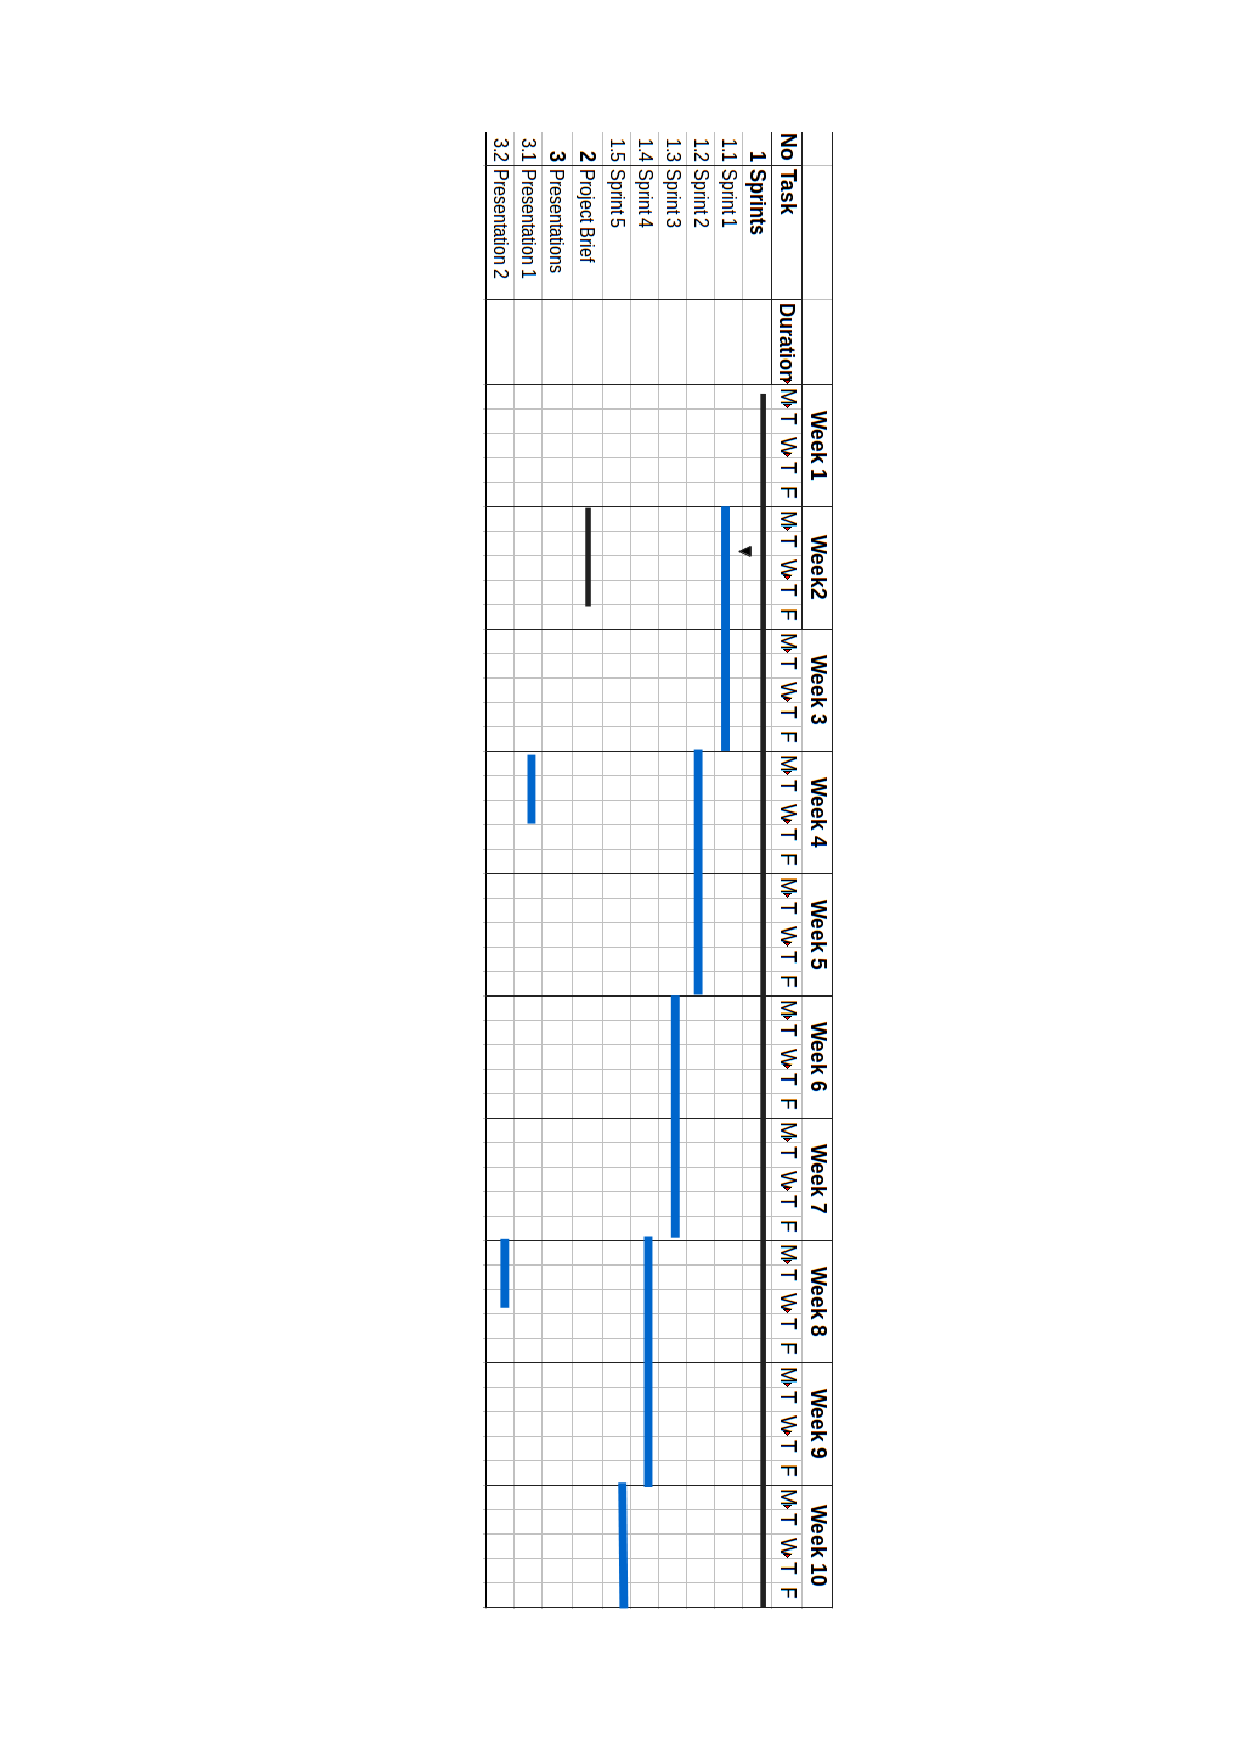
\includegraphics[scale=0.8]{GanttChart.pdf}
\end{center}

\section{Feedback email from Adrian McKenzie}

Hi guys\\
As discussed, some feedback for you from Eddie and myself.
\\\\
The deliverables produced from your Group Design Project have resulted in a good outcome for Snowflake Software; they answered some of our key questions and provided a solid foundation to commence our Pub-Sub product development in 2015. 
\\\\
The project posed some significant challenges including reconciling complex technical standards with the user requirements and a complex set of factors to weigh up in selecting the technologies to use. Reaching firm conclusions about the relative merits of the technologies you assessed represents a real achievement. 
\\\\
As mentioned during the wrap up from the final demonstration I feel it would have been productive if there was a more balanced contribution to Sprint planning, demonstration and retrospectives from each member of the team.
\\\\
If possible we would like a copy of your group report and individual reflections to further understand your view of what happened within the project, so that we can improve the experience for next year's group.
\\\\
We enjoyed collaborating with you and are hopeful that it was a positive experience that has helped you understand something of the software industry.
\\\\
If any of you are interested in exploring the possibility of joining us at Snowflake Software I would be more than happy to catch-up for an informal conversation.
\\\\
Good luck for the end of your degree and future career.
\\\\
Adrian\\
-- \\
Adrian McKenzie\\
Head of Software Development\\
Snowflake Software 


\end{document}
